\subsubsection{LiteDB Pipeline} \label{sec:ExperimentePIPE}
    Um die Suche von mehreren Paketen in der Datenbasis zu beschleunigen wurde sich das Prinzip der Parallelisierung zu Nutzen gemacht.
    Hierzu wurde die zu untersuchende Liste von Paketen auf verschiedene Tasks aufgeteilt.
    So ist nach dem vollständigen Befüllen der Pipeline eine theoretischen Laufzeitverkürzung um der Faktor der maximal abarbeitbaren Tasks erreicht.  
    
    Dabei sind zwei Fälle zu unterscheiden:
    \begin{description}
        \item[\textit{Weniger} Pakete als Datenbank-Dateien]\hfill \\
            In diesem Falle einer geringeren Anzahl an Pakete wird die Pipe nie vollständig gefüllt.
        \item[\textit{Mehr} Pakete als Datenbank-Dateien]\hfill \\
            In jenem Falle muss die Paketliste Stück für Stück in die Pipe eingefügt werden und beim Erreichen der Kapazität -- entsprechend der Anzahl der Datenbanken -- das früheste Paket entfernt und ein neues Paket am Anfang eingefügt werden.
    \end{description}
    
    Die Verwaltung der 3 verschiedenen Staaten der Pipe ist in folgender Abbildung mit \ac{PAP} nachvollziehbar.
    Anschließend sind die 3 Fälle näher ausgeführt.
    \begin{figure}[H]
        \centering
        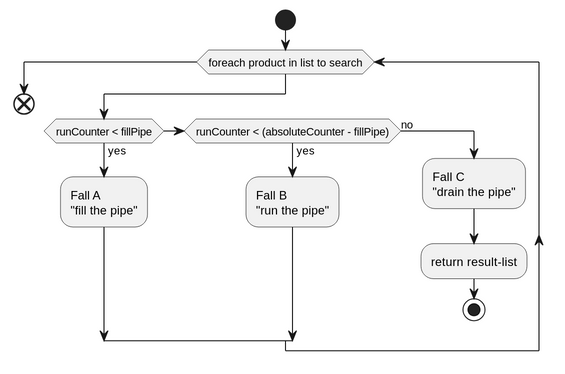
\includegraphics[width=\textwidth]{../pap/Simultanius search on LiteDb-Files_k.png}
        \caption{Übersicht der Pipeline-Staaten}
        \label{png:OverviewPipelineStatus}
    \end{figure}

    \newpage
    Das Befüllen der Pipeline geschieht nach folgendem Muster:
    \begin{figure}[H]
        \centering
        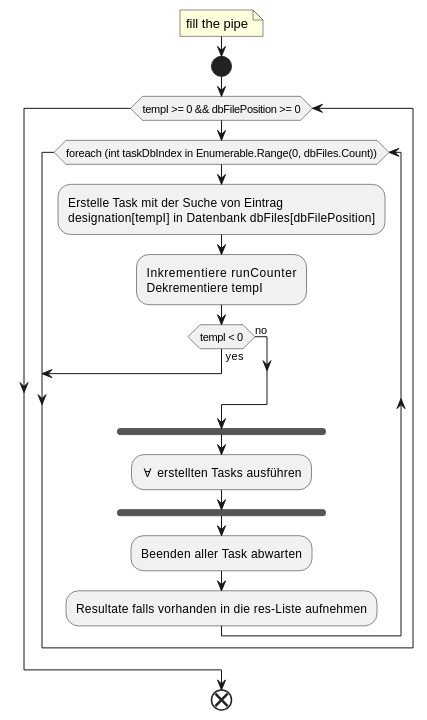
\includegraphics[width=0.75\textwidth]{../pap/Case_A_k.png}
        \caption{\ac{PAP} Befüllen der Pipeline}
        \label{png:case_a}
    \end{figure}
    Zu Erkennen ist, dass solange ein neuer Task erstellt wird, wie die Anzahl erstens nicht die Anzahl der Datenbanken erreicht hat und zweitens die aktuelle Anzahl an Tasks nicht über dem Wert der Datenbankenmenge ist.
    Dies definiert das Befüllen der Pipe.

    \newpage
    Nach vollständiger Befüllung die Erhaltung der Pipeline:
    \begin{figure}[H]
        \centering
        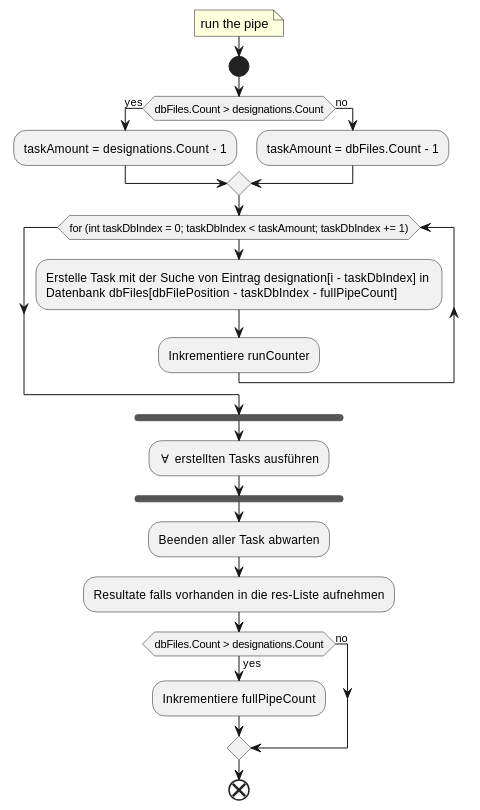
\includegraphics[width=0.75\textwidth]{../pap/Case_B_k.png}
        \caption{\ac{PAP} Aufrechterhalten der Pipeline}
        \label{png:case_b}
    \end{figure}
    Hier wird jetzt nachdem das älteste, am zeitigsten in der Pipe eingeführte und noch zu analysierende Paket aus der Liste entfernt und am Anfang der Datenbankenliste der nächste Eintrag wieder angeführt, um ebenfalls alle Datenbanken zu durchlaufen.
    \\
    Dieser Prozess wird nur dadurch unterbunden, wenn der Zähler registriert, dass keine größere Zahl an noch zu analysierenden Paketen als Datenbankdateien wartend ist und somit das entleeren der Pipe eingeläutet werden muss.

    \newpage
    Beim Leeren der Pipeline:
    \begin{figure}[H]
        \centering
        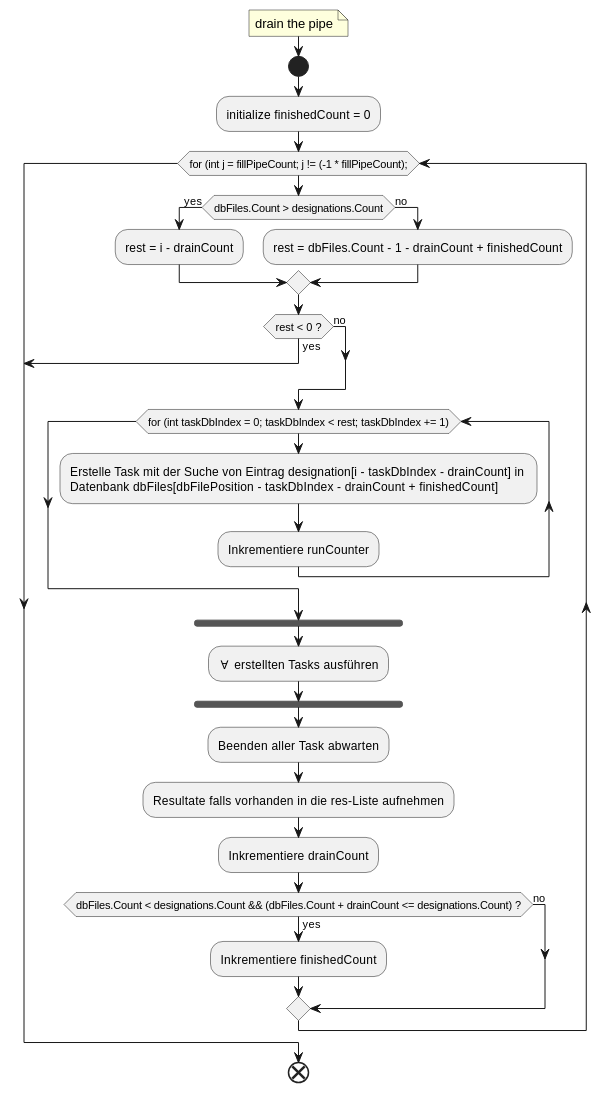
\includegraphics[width=0.75\textwidth]{../pap/Case_C_k.png}
        \caption{\ac{PAP} Leeren der Pipeline}
        \label{png:case_c}
    \end{figure}
    Hier wird beim vollständigen Durchlaufen eines Paketes dieses entfernt aus der Liste und alle weiteren rücken eine Eintrag nach vorne, wodurch die letzten Pakete ebenfalls noch durch die restlichen Datenbankdateien vollständig abgeglichen werden.

    \newpage
    Aus der Implementation der Pipeline ergeben sich folgende Laufzeiten bei weniger Paketen als Datenbankdateien:\\
    \begin{tabularx}{0.8\textwidth}{|c|c|c|}
        \hline
        Such-Typ & Zeit & Faktor \\ \hline
        Mono-Suche & 262676.7ms & 1 \\
        Pipeline & 96868.4ms & 2.7213448 \\
        \hline
        \caption{Laufzeiten Durchschnitt 10 Messungen -- Weniger Pakete als Datenbankdateien \textsuperscript{siehe Appendix \ref{subsec:ZeitunterschiedAbfrageAufDenDatenbankenMonoPipeFallWenigerPaketeAlsDatenbanken}}}
        \label{tabularx:LessPackagesThenDbFiles}
    \end{tabularx}

    Aus der Implementation der Pipeline ergeben sich folgende Laufzeiten bei mehr Paketen als Datenbankdateien:\\
    \begin{tabularx}{0.8\textwidth}{|c|c|c|}
        \hline
        Such-Typ & Zeit & Faktor \\ \hline
        Mono-Suche & 95011.24ms & 1 \\
        Pipeline & 22111.5ms & 4.296846569 \\
        \hline
        \caption{Laufzeiten Durchschnitt 10 Messungen -- Weniger Pakete als Datenbankdateien \textsuperscript{siehe Appendix \ref{subsec:ZeitunterschiedAbfrageAufDenDatenbankenMonoPipeFallMehrPaketeAlsDatenbanken}}}
        \label{tabularx:MorePackagesThenDbFiles}
    \end{tabularx}
    Deutlich ablesbar ist in den Tabellen \ref{tabularx:LessPackagesThenDbFiles} und \ref{tabularx:MorePackagesThenDbFiles}, dass jeweils ein Zeitgewinn erzielt wurde.
    Somit ist die Pipeline eine deutliche Verbesserung für die Antwortzeiten des Webservices.
